\documentclass[11pt]{amsart}
\usepackage{amssymb,amsmath,amsthm,mathtools}
\usepackage[utf8]{inputenc}
\usepackage{tikz}
\usepgflibrary{patterns}
\usepgflibrary[patterns]
\usetikzlibrary{patterns}
\usetikzlibrary[patterns]
\usepackage{color}
\usepackage{xcolor}

\begin{document}

	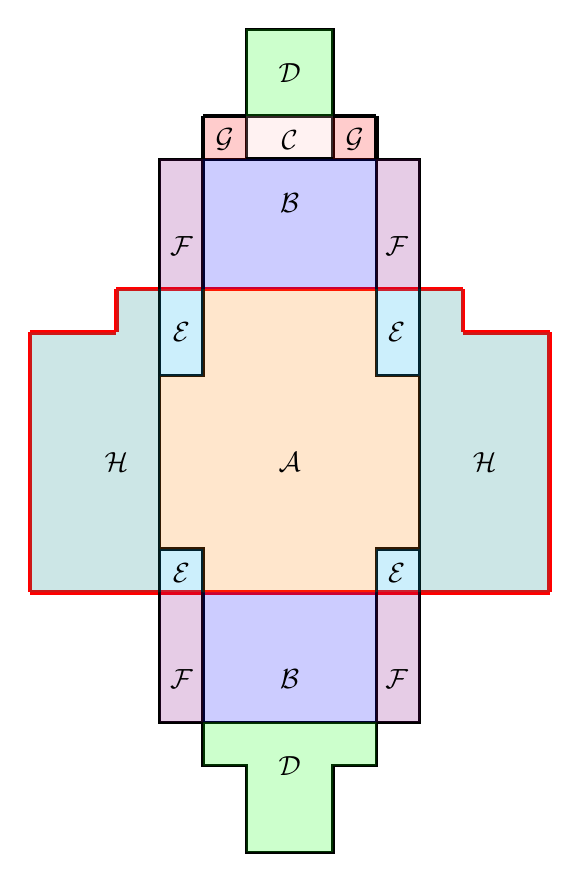
\begin{tikzpicture}[scale=0.55]
		\draw[red,ultra thick] 
		(-16,-3) -- (-4,-3);
		\draw[red,ultra thick]
		(-16,3) -- (-14,3);
		\draw[red,ultra thick]
		(-14,3) -- (-14,4);
		\draw[red,ultra thick]
		(-14,4) -- (-6,4);
		\draw[red,ultra thick]
		(-6,4) -- (-6,3);
		\draw[red,ultra thick] 
		(-6,3) -- (-4,3);
		\draw[red,ultra thick]
		(-4,3) -- (-4,-3);
		\draw[red,ultra thick]
		(-16,3) -- (-16,-3);
		%competitor
		\draw[black,very thick] 
		(-9,-9)--(-9,-7)--(-8,-7)--(-8,-2)--(-7,-2)--(-7,2)--(-8,2)--(-8,7)--(-9,7)--(-9,10)--(-11,10)--(-11,7)--(-12,7)--(-12,2)--(-13,2)--(-13,-2)--(-12,-2)--(-12,-7)--(-11,-7)--(-11,-9)-- cycle;
		%soluzione
		\draw[black,very thick] 
		(-7,-6)--(-7,7)--(-9,7)--(-9,8)--(-11,8)--(-11,7)--(-13,7)--(-13,-6)-- cycle;
		%colori verde D
		\fill[green, opacity=0.2] (-8,-6)--(-8,-7)--(-9,-7)--(-9,-9)--(-11,-9)--(-11,-7)--(-12,-7)--(-12,-6)--cycle;
		\fill[green, opacity=0.2] (-11,8)--(-9,8)--(-9,10)--(-11,10)--cycle;
		\draw [black ,ultra thick]     (-10,9) node{$\mathcal{D} $};
		\draw [black ,ultra thick]     (-10,-7) node{$\mathcal{D} $};
		%colori rosa C
		\fill[pink, opacity=0.2] (-11,8)--(-9,8)--(-9,7)--(-11,7)--cycle;
		\draw [black ,ultra thick]     (-10,7.45) node{$\mathcal{C} $};
		\draw [black ,ultra thick] (-11,7) -- (-9,7);
		%colori G rosso
		\fill[red, opacity=0.2] (-11,7)--(-11,8)--(-12,8)--(-12,7)--cycle;
		\fill[red, opacity=0.2] (-9,7)--(-9,8)--(-8,8)--(-8,7)--cycle;
		\draw [black ,ultra thick] (-12,7) -- (-12,8);
		\draw [black ,ultra thick] (-8,8) -- (-8,7);
		\draw [black ,ultra thick] (-9,8) -- (-8,8);
		\draw [black ,ultra thick] (-12,8) -- (-11,8);
		\draw [black ,ultra thick]     (-8.5,7.45) node{$\mathcal{G} $};
		\draw [black ,ultra thick]     (-11.5,7.45) node{$\mathcal{G} $};
		% colori B blue
		\fill[blue, opacity=0.2] (-12,7)--(-12,4)--(-8,4)--(-8,7)--cycle;
		\fill[blue, opacity=0.2] (-12,-3)--(-12,-6)--(-8,-6)--(-8,-3)--cycle;
		\draw [black ,ultra thick]     (-10,6) node{$\mathcal{B} $};
		\draw [black ,ultra thick]     (-10,-5) node{$\mathcal{B} $};
		%colori F viola
		\fill[violet, opacity=0.2] (-12,-3)--(-13,-3)--(-13,-6)--(-12,-6)--cycle;
		\fill[violet, opacity=0.2] (-12,4)--(-13,4)--(-13,7)--(-12,7)--cycle;
		\fill[violet, opacity=0.2] (-8,-3)--(-7,-3)--(-7,-6)--(-8,-6)--cycle;
		\fill[violet, opacity=0.2] (-8,4)--(-7,4)--(-7,7)--(-8,7)--cycle;
		\draw [black ,ultra thick]     (-7.531,-5) node{$\mathcal{F} $};
		\draw [black ,ultra thick]     (-7.531,5) node{$\mathcal{F} $};
		\draw [black ,ultra thick]     (-12.5,-5) node{$\mathcal{F} $};
		\draw [black ,ultra thick]     (-12.5,5) node{$\mathcal{F} $};
		% colori E azzurro
		\fill[cyan, opacity=0.2] (-12,-3)--(-13,-3)--(-13,-2)--(-12,-2)--cycle;
		\fill[cyan, opacity=0.2] (-12,4)--(-13,4)--(-13,2)--(-12,2)--cycle;
		\fill[cyan, opacity=0.2] (-8,-3)--(-7,-3)--(-7,-2)--(-8,-2)--cycle;
		\fill[cyan, opacity=0.2] (-8,4)--(-7,4)--(-7,2)--(-8,2)--cycle;
		\draw [black ,ultra thick]     (-7.531,3) node{$\mathcal{E} $};
		\draw [black ,ultra thick]     (-12.5,-2.56) node{$\mathcal{E} $};
		\draw [black ,ultra thick]     (-12.5,3) node{$\mathcal{E} $};
		\draw [black ,ultra thick]     (-7.531,-2.56) node{$\mathcal{E} $};
		% colori A arancione
		\fill[orange, opacity=0.2] (-8,4)--(-12,4)--(-12,2)--(-13,2)--(-13,-2)--(-12,-2)--(-12,-3)--(-8,-3)--(-8,-2)--(-7,-2)--(-7,2)--(-8,2)--cycle;
		\draw [black ,ultra thick]     (-10,0) node{$\mathcal{A} $};
		% colori H verde acqua
		\fill[teal, opacity=0.2] (-16,-3)--(-16,3)--(-14,3)--(-14,4)--(-13,4)--(-13,-3)--cycle;
		\fill[teal, opacity=0.2] (-7,-3)--(-7,4)--(-6,4)--(-6,3)--(-4,3)--(-4,-3)--cycle;
		\draw [black ,ultra thick]     (-14,0) node{$\mathcal{H} $};
		\draw [black ,ultra thick]     (-5.5,0) node{$\mathcal{H} $};

	\end{tikzpicture}

\end{document}